


\section{Introduction}



Information collection processes are growing in quantity as a
consequence of the emergence of embedded systems and sensor networks.
Nowadays it is possible to collect large amounts of data to monitor
and control complex systems.  This information must be analysed and
prepared by information systems in order to detect eventual sensor
failures or malfunctions and, if it is possible, to reconstruct the
incorrect signals. Acquired data instance are bound to a timestamp,
therefore correctness criteria must include both data value and its
timestamp. The sequences of data values collected at specific
timestamps are formalised as time series.


Time series are defined as a collection of observations made
chronologically.  In general, time series come from a continuous
nature in which they are recorded at regular intervals, such as hourly
or daily, or at irregular intervals, such as recording when a pump is
open or closed.  One problem when dealing with time series data
results from the fact that these data are often voluminous
\cite{fu11,keogh08:isax}, as a result, efficiently storing and
accessing them can be complex. Moreover, this is specially critical
when developing small embedded systems, whose resources (capacity,
energy, processing and communications) suffer restrictions
\cite{yaogehrke02}.  Another problem is that the procedure of
processing and synthesising information becomes difficult if data is
not equi-time spaced.



Time series can be stored and managed by Structured Query Language
(\acro{SQL}) relational database management systems. However, some
authors \cite{dreyer94,schmidt95,stonebraker09:scidb,zhang11} notice
that the use of \acro{SQL} systems as a time series backend suffers
some drawbacks.  On the one hand, \emph{NoSQL} or \emph{NewSQL}
products are being developed in order to increase the performance and
flexibility of \acro{SQL} systems
\cite{atzeni13:relational_model_dead,stonebraker10,stonebraker09:scidb,zhang11},
however the continue acquisition nature of time series is an issue for
storing and analysing offline all the data \cite{keogh97}.

On the other hand, compression techniques for time series are
considered in the form of approximation to the original signal in
order to compute analysis such as similarity or pattern search
\cite{fu11,keogh01,last01} or in the form of compression and
aggregation approaches for massive data streams
\cite{cormode08:pods,bonnet01}. However, treating time series as data
streams does not consider adequately the time dimension nor computes
the evolution of aggregated parameters along time, which is
interesting for monitoring purposes.  On a similar approach,
\emph{RRDtool} \cite{rrdtool} is a system that stores time series
aggregated in different resolutions in order to compact data and to do
faster visualisations. However, \emph{RRDtool} is very specific and
has limited aggregation operations to applications of network
counters.



\subsection{Contribution}


%TSMS

This paper focuses on Data Base Management Systems \linebreak[4]
(\acro{DBMS}) that store and treat data as time series, usually known
as Time Series Data Base Management Systems (\acro{TSMS}),
\cite{dreyer94,last01}.  We introduce a new data model named
multiresolution \acro{TSMS} (\acro{MTSMS}). This model organises data
in an aggregated way and  allows to store time series using
different time resolutions. It is designed to cope well with bounded
storage computers such as sensor systems.  

We describe the model in two separated submodels, one \acro{TSMS}
model mainly for describing time series basic concepts and operations
and the other a \acro{MTSMS} model for describing multiresolution over
time series. The model is described firmly rooted on set and
relational algebra as a formal theory for information systems.  It
also considers the time irregularities sampling of time series,
moreover it operates coherently with the time dimension of time
series.


% Our multiresolution definition is
% based on concepts of RRDtool but aims to generic applications and has
% more generic operators.


Multiresolution is proposed as a lossy storage solution that selects
only the needed information. The concept is similar to multimedia
lossy compression methods, where information can be discarded in
favour of size, but applied to time series.  Multiresolution is an
aggregation of data that stores the evolution of the parameters along
time, which is more related to the needs of monitoring. However, as a
lossy storage solution, the multiresolution schema has to be decided
for each application, deciding what approximate queries will be needed
to resolve. We formalise aggregation functions as an independent
object of the main model. Therefore, users can define new operations
and other aggregation methods from other fields such as data
streaming or time series data mining.


A representation function concept of time series is also formalised, then
users can define different operators considering the behaviour of time
series in different contexts. Especially, it is important when defining
new aggregation operations that must consider different meanings of
the time series, i.e. \emph{RRDtool} specific counter time series
aggregations. Furthermore, we formalise representation as an
independent object of the main model.




\subsection{Outline}

This manuscript is organised as follows.  In
Section~\ref{sec:related-work} some related work concerning
\acro{TSMS} and \acro{MTSMS} are presented.  The motivation for
multiresolution is shown in Section~\ref{sec:features}.  The
\acro{TSMS} model is presented in Section~\ref{sec:model:TSMS} and the
\acro{MTSMS} model is presented in Section~\ref{sec:MTSMS}.  In
Section~\ref{sec:implementation} there is a implementation
for the \acro{TSMS}+\acro{MTSMS} model.  Section~\ref{sec:example} is
devoted to a real data multiresolution database example.  Finally,
Section~\ref{sec:concl-future-work} offers some conclusions.
\ref{sec:notation} shows main notation symbols.





\section{State of the art}
\label{sec:related-work}

In this section, related work to mutiresolution time series is
described in three parts: some database management systems
approaches for time series, compression techniques applied to time
series, and computations based on data streams.




\subsection{Database approaches}

Some authors treat \acro{TSMS} as a particular \acro{DBMS} field
\cite{last01}.  Segev and Shoshani \cite{segev87:sigmod} propose an
structured language for querying \acro{TSMS}. Their time series
structures include the notion of regularity and temporal
representation and their operations are \acro{SQL}-like.  Dreyer et
al.\ \cite{dreyer94} propose the requirements of special purpose
\acro{TSMS} and base the model on five basic structural elements:
events, time series, groups, metadata and time series bases. They
implement a \acro{TSMS} called \emph{Calanda} which includes calendar
operations, allows grouping time series and operating with simple
queries. They exemplify it with financial data. In \cite{schmidt95}
\emph{Calanda} is compared with temporal systems designed for time
series.



 
Others implement \acro{TSMS} with array database approaches.
\emph{SciDB} \cite{stonebraker09:scidb} and \emph{SciQL}
\cite{zhang11} are array database systems intended for science
applications, in which time series play a principal role. They
structure time series into arrays in order to achieve multidimensional
analysis and they store other data into tables.  \emph{SciDB} is based
on arrays which, according to the authors, allow to represent time
series.  In contrast, \emph{SciQL} defines time series as a mixture of
array, set, and sequence properties and exhibits some time series
managing characteristics that include time series regularities,
interpolation or correlation queries.
% However,
% difference between tables and arrays seems too physical and leads to
% ambiguity when representing time series.  
% Our TSMS model proposes time
% series as firmly based on relational algebra, clarifying this
% ambiguity and describing them coherently in terms of information
% systems theory.





Bitemporal \acro{DBMS}, sometimes referred directly as temporal data,
is a database field related with time. Bitemporal data manages
historical data and events in databases by associating pairs of
\emph{valid} and \emph{transaction} time intervals to data.
Bitemporal data and time series data are not exactly the same and so
can not be treated interchangeably \cite{schmidt95}, however, there
are some similarities that can be considered. Moreover, \acro{DBMS}
research represents bitemporal data as relations extended with time
intervals attributes and extends relational operations in order to
deal with related time aspects
\cite{jensen99:temporaldata,date02:_tempor_data_relat_model}.  We
formalise time series similarly as how bitemporal data is formalised
for relational \acro{DBMS}.
% On the other hand, some bitemporal time concepts might be taken
% into account by \acro{TSMS}, such as the discussions about time
% granularities.



\subsection{Compression techniques}


% As \acro{TSMS} suffer from problematic properties of time
% series, like the ones we describe in
% Section~\ref{sec:model:properties} mainly the huge data volume,
% compression techniques are used.  Next, we summarise some current work
% in \acro{TSMS} with compression.



\emph{RRDtool} from Oetiker, \cite{rrdtool,lisa98:oetiker}, is a free
software database management system. It is designed to be used for
monitoring systems. Because of this, it is focused to a particular
kind of data, gauges and counters, and it lacks general time series
operations. \emph{RRDtool} can store multiple time resolution data,
however Plonka et al.\ \cite{lisa07:plonka} evaluated \emph{RRDtool}
performance and found limitations when storing huge number of
different time series. They propose a caching system on top of
\emph{RRDtool} as a solution.  \emph{RRDtool} is extremely used by the
free software community so it inspired us to develop a model from its
main characteristics, that is now what we call multiresolution. A
similar approach is done by \cite{weigel10} in a system called
\emph{TSDS} that caches queries by aggregate parameters. They notice
that data needs to be shown over its full time range and not only
subsets of data as it is usually provided.  They develop the software
package \emph{TSDS} where time series are stored fully and then
requested by date ranges or by applying different filters and
operations to the time series data.  Our \acro{MTSMS} model is a generic
approach to the multiresolution features, we define it open so that
users can define any attribute aggregate functions.


Deri et al.\ \cite{deri12:tsdb_compressed_database} present
\emph{Tsdb}, a lossless compression storage \acro{TSMS} for time
series that share the same time instants of acquisition. Different
time series are stored grouped by the time of acquisition instead of
each time series isolated.  They compare \emph{Tsdb} with \emph{RRDtool} and
with a relational product. As a consequence of \emph{Tsdb} structure,
they achieve a better measure addition time but a worse global
retrieval time as data has to be contiguously regrouped. However, when
measures have same time this is seen as the same time series in a
\acro{MTSMS}, so it would be interesting to use this implementation
architecture of shared time arrays in \acro{MTSMS} for resolution subseries
with same delta time in order to achieve better performance requirements
when having much equal acquired time series.

% Therefore, as it is a very different approach from RRDtool we find it difficult to compare both in these performance requirements. 
% He only evaluates compression performance but we think that a global
% evaluation of compression plus descompression must be done. MTSMS
% are not aimed to be a replacement for offline long time storage
% systems that are rarely queried and then queries can be slow but
% have tot be exact. MTSMS are adequate to stream processing and
% resolving queries with less data than original and so they are
% quicker but give information previously selected.


There are other lossy compression techniques for time series devoted
to the optimal approximation representation, that is finding the
compromise between least data that can reconstruct the original signal
with least error. Keogh et al.\ \cite{keogh01} cite some possible
approximation representations for time series such as Fourier
transforms, wavelets, symbolic mappings or piecewise linear
representation. They remark this last one as very usual due to its
simplicity and develop a system called \emph{iSAX}
\cite{keogh08:isax,keogh10:isax} in order to analyse and index massive
collections of time series. They describe that the main problem is in
the indexing of time series and they propose methods for processing
efficiently. The first method proposed is based on a constant
piecewise approximation. The time series representation obtained with
\emph{iSAX} allows reducing the stored space and indexing faster with
the same quality as other more complex representation methods.  These
compression techniques are candidates for being used as attribute
aggregate functions in the \acro{MTSMS} model, as instance it would be
interesting to define aggregations in the frequency domain of time
series.


% A Multiresolution Symbolic Representation of
% Time Series; Megalooikonomou, Faloutsos; 2005 proposes multiresolution by decomposing a signal in frequency subsequences and intended mainly to similarity searching. The objective is to reconstruct the original time series. 
 


% \paragraph{T-Time}  \textcite{assfalg08:thesis} shows a TSMS that can do similarity search, which is calculated as distances between time series. Mainly, two time series are marked as similar if they distance is less than a threshold in each interval. From this method efficient algorithms are developed and implemented in a program called T-Time, which is described in \cite{assfalg08:ttime}.

 


\subsection{Data stream}



There are other \acro{TSMS} specifically designed for a particular
field requirements.  \emph{Cougar} \cite{bonnet01} is a sensor
database system that has two main structures: one for sensor
properties stored into relational tables and another for time series
stored into data sequences from sensors. Time series have specific
operations and can combine relations and sequences. \emph{Cougar}
target field is sensor networks, where data is stored distributed in
different locations. Queries are resolved combining sensor data in a
data stream abstraction that improves processing performance.

Time series as data streams are also considered when aggregating
statistically data in order to do fast approximate queries with
compressed data. Cormode et al.\ \cite{cormode08:pods} develop
aggregation techniques that consider giving more weight to recent
information.  Our \acro{MTSMS} model applies a similar approach of
weighting more recent data but specifically to time series, with
multiple aggregations and considering time irregularities.  Dou et
al.\ \cite{dou14:historic_queries_flash_storage} create index
structures as multiresolution aggregates, like average, count, or top,
for historical data managed in flash storage; they consider a specific
storage solution based on register with pointers similar to the
multiresolution storage in \emph{RRDtool} \cite{lisa98:oetiker}.

% Our MTSMS model can also be thought as an stream processor if measures
% are added in time order, there is no possibility of update operations,
% buffer time series become of unity cardinality, and aggregate
% functions are limited to stream capabilities ones.  
% As instance,
% RRDtool can be considered stream oriented and its consolidation
% process is done at the same time of inserting new measures.





\section{Multiresolution motivation}
\label{sec:features}

A \acro{TSMS} is a special purpose \acro{DBMS} devoted to store and
manage time series.  The main objective of \acro{TSMS} is to gather
two areas of study: time series analysis and \acro{DBMS}.  Time series
analysis formalises a great amount of algorithms and methodologies
that apply to time series, with a main focus on improving
efficiency. \acro{DBMS} theory formalises systems that store and
operate with data, currently the relational model is the referent
\cite{date:introduction}.



In time series analysis there are some common generic operations.
Most of these operations deal with the time given the nature of data.
Usual operations include querying time intervals, finding time
correlations, or calculating distances between two time series. In
all these operations \acro{TSMS} must consider the temporal coherence
of the time series.  In the context of statistics, aggregation of time
series is also a common operation. Aggregate means to summarise a time
series subset by a smaller set of measures. Statistic indicators like
the mean, the maximum, or the mode, for instance, summarise time
series into one only measure.

In the discrete context, a time series is defined as a set of value
and time pairs. Furthermore, a time series has a continuous nature as
it comes from a phenomena evolution along time. As a result,
\acro{TSMS} operations may deal with this time series nature by
methods of interpolation or approximation.


A \acro{MTSMS} proposes a \acro{TSMS} with multiresolution
capabilities.  A \acro{MTSMS} schema represents a time series using a
set of different resolutions.  The multiresolution concept comes from
thoroughly analysis of \emph{RRDtool} \cite{rrdtool}. Our objectives
have been to formalise the main concepts into an abstract model and to
include more genericity in order to describe \acro{MTSMS} as fully
\acro{TSMS}.

%Then we will be able to apply these systems to other applications.

As a summary, \acro{MTSMS} improve \acro{TSMS} features in various aspects:
\begin{itemize}

\item Voluminous data. Monitoring systems capture a huge amount of
  data from sensors. In order to be able to process this information,
  data volume must be reduced. One of the features of the
  multiresolution approach is to select and store only the most
  interesting segments of data. This segments are seen as different
  resolutions for the same time series and the user can configure how
  they are extracted and summarised by defining different time steps
  and functions. Multiresolution can also be useful when graphing time
  series allowing the user to select the best time range and time
  step that fits into the screen; there is no need to process with
  more quantity of data than the one that can be
  shown.% In figure~\ref{fig:mtsms:sequence} there is an example of
  % extracting two resolutions: one every three units of time and
  % another every five.

\item Data validation. Monitoring systems capture data but can occur
  some drawbacks that will affect later the process of time series
  analysis. Main problems are found when monitors can not capture
  data, known as gaps, or capture data erroneously, such as outlayers
  \cite{quevedo10}.  The multiresolution attribute functions is
  designed to cope well with validating, filtering and reconstructing
  with this unknown data in order to keep a consistent
  historic.% In figure~\ref{fig:mtsms:sequence-irregular} an
  % example of a gap can be seen.

\item Data time regularising. Another monitoring side effect happens
  when the sampling rate is not constant, that is when the resulting
  data is not equi-time spaced. This no regularities can come from
  sampling jitters in periodic sampling or from no periodic
  event-based sampling \cite{kopetz11:realtime}. One multiresolution
  consolidation objective is to regularise the time interval when
  processing a time series, therefore each resulting time series
  segment has a regular time resolution. This regularising approach
  could also be used when the user wants to consult another resolution
  for a time series, such as changing periodic data from a month to a
  year step. % In
  % figure~\ref{fig:mtsms:sequence-irregular} an example of time
  % regularising can be seen.

\item Information summaries. Time series analysis typically focuses on
  reconstructing the original signal. However, the user objective in a
  database system is to consult some information. The multiresolution
  approach allows a lossy compression storage solution for data. Therefore
  it can be regarded as to extracting the interesting information and
  then storing it. The selected information must be determined a
  priori assuming the context where the future queries will be done.
  % In
  % figure~\ref{fig:mtsms:sequence} there is an example of summarising by
  % mean attribute.
\end{itemize}


However sometimes it may also be useful to complement \acro{MTSMS}
with other \acro{DBMS}. Not only to store the original values as a
long-term deposit consulted offline, but also to store related
information to time series such as units of values, sensor
localisation, classification tags, last measured value, etc.



\subsection{Motivation example}

Figure~\ref{fig:mtsms:sequence} shows an example of a multiresolution
summary for a time series. It shows a snapshot in time, suppose
between time 9 and 10. At the top of the figure there is a plot of a
time series with time axis in general units of time (u.t.) and with
value axis in undetermined units. The 'now' point shows when the
snapshot has been taken, so the time before is the past and the time
after is the future, which is grey coloured. The \emph{init} point
shows when the database system has started sampling, so data in time
before is unknown; the starting point is indicated as zero u.t.\ and
the earlier unknown time points have negative units.


\begin{figure}
  \centering
  \tikzsetnextfilename{fig_mtsms_sequence}
  %\usetikzlibrary{positioning}
\begin{tikzpicture}[scale=0.77, every node/.style={transform shape}]

  %referencia
  \node (-6) {};

  \foreach \x in {-5,...,12}
  {
    \pgfkeys{/pgf/number format/.cd,int trunc}
    \pgfmathparse{abs(\x)}
    \let\absx=\pgfmathresult
    \pgfmathparse{\x-1}
    \let\antx=\pgfmathresult
    %time
    \node[node distance=1mm] (\x) [right=of \antx] 
    {\ifnum\x<11 \x \else \phantom{9} \fi};

    %graph values
    \node [above=\absx mm of \x] 
    {\ifnum\x=10 \color{gray} \fi \ifnum\x<11 $\bullet$ \fi};    

    %values
    % \node[rectangle,draw] (s\x) [below=of \x] 
    % {\ifnum\x<10 \pgfmathprintnumber{\absx} \else \phantom{9} \fi};
    \ifnum\x<10
    \node[rectangle,draw] (s\x) [below=of \x] 
    {\pgfmathprintnumber{\absx}};
    \else
    \node[rectangle,dotted,draw] (s\x) [below=of \x] 
    {\phantom{9}};
    \fi
  }

  \node [below=of 10] {\color{gray}10}; 
  

  
  %rd: 5s |inf| mean
  \node [circle,draw] (rd5-5) [below=3cm of s-5] {u};
  \node [circle,draw] (rd50) [below=3cm of s0] {u};
  \node [circle,draw] (rd55) [below=3cm of s5] {3};
  \node [circle,dotted,draw] (rd510) [below=3cm of s10] {\color{gray}u};
  \node [below=3.3cm of s10] {\color{gray}8};
 
  \draw[->,bend right] (s5) to (rd55);
  \draw[->,bend right] (s4) to (rd55);
  \draw[->,bend right] (s3) to (rd55);
  \draw[->,bend right] (s2) to (rd55);
  \draw[->,bend right] (s1) to (rd55);

  \draw[->,dotted,bend right] (s10) to (rd510);
  \draw[->,bend right] (s9) to (rd510);
  \draw[->,bend right] (s8) to (rd510);
  \draw[->,bend right] (s7) to (rd510);
  \draw[->,bend right] (s6) to (rd510);

  
  %rd: 3s |inf| mean
  \node [circle,draw] (rd3-3) [below=of s-3] {u};
  \node [circle,draw] (rd30) [below=of s0] {u};
  \node [circle,draw,fill=white] (rd33) [below=of s3] {2};
  \node [circle,draw,fill=white] (rd36) [below=of s6] {5};
  \node [circle,draw,fill=white] (rd39) [below=of s9] {8};
  \node [circle,dotted,draw] (rd312) [below=of s12] {\color{gray}u};

  \draw[->] (s3) to (rd33);
  \draw[->] (s2) to (rd33);
  \draw[->] (s1) to (rd33);

  \draw[->] (s6) to (rd36);
  \draw[->] (s5) to (rd36);
  \draw[->] (s4) to (rd36);

  \draw[->] (s9) to (rd39);
  \draw[->] (s8) to (rd39);
  \draw[->] (s7) to (rd39);

  \draw[->,dotted] (s12) to (rd312);
  \draw[->,dotted] (s11) to (rd312);
  \draw[->,dotted] (s10) to (rd312);



  %eixos
  \node (et0) [above=1mm of -5] {};
  \node (et12) [above=1mm of 11] {};
  \node [right=-2mm of et12] {time};
  \draw[->] (et0) to (et12);
  \node (y5) [above=5mm of 0] {--};
  \node [left=-1.5mm of y5] {5};
  \node (y10) [above=10mm of 0] {--};
  \node [left=-1.5mm of y10] {10};

  \node (inici) [above=4cm of s0] {init};
  \node (inici2) [below=4cm of s0] {};
  \draw[-,dotted] (inici) to (inici2);

  \node (fi) [above=4.4cm of s9.east] {now};
  \node (fi2) [below=4.4cm of s9.east] {};
  \draw[-,dotted] (fi) to (fi2);


  \node (fut) [below right=1mm and 1mm of fi] {future};
  \draw[->] (fut.south west) to (fut.south east);

  \node (pas) [below left=1mm and 1mm of fi] {past};
  \draw[->] (pas.south east) to (pas.south west);

  \node (unk) [below left=1mm and 1mm of inici] {unknown};
  \draw[->] (unk.south east) to (unk.south west);



  \node [above=0cm of s-5] {\makebox[0cm][l]{sample every 1 u.t.}};
  \node [below=0.5cm of s-5] {\makebox[0cm][l]{mean every 3 u.t.}};
  \node [below=2.5cm of s-5] {\makebox[0cm][l]{mean every 5 u.t.}};


\end{tikzpicture}



%%% Local Variables:
%%% TeX-master: "../main"
%%% ispell-local-dictionary: "british"
%%% End:

  %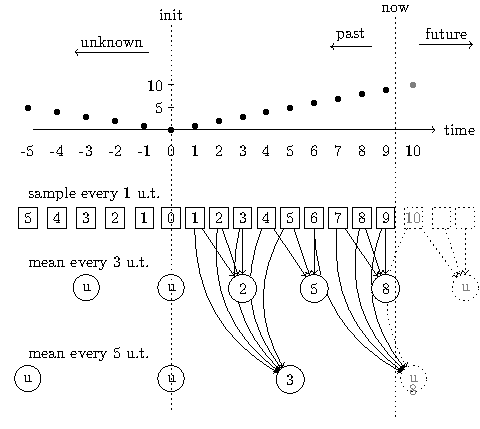
\includegraphics{fig/fig_mtsms_sequence}
  \caption{Multiresolution snapshot diagram with regular sampling}
  \label{fig:mtsms:sequence}
\end{figure}


% \begin{figure}[tp]
%   \centering
%   %\usetikzlibrary{positioning}
\begin{tikzpicture}

  \node[node distance=1mm] (0) {0};
  \node[node distance=1mm] (-1) [left=of 0]{\phantom{9}};
  \node[node distance=1mm] (1) [right=of 0] {\phantom{1}};
  \node[node distance=1mm] (2) [right=of 1] {2};
  \node[node distance=1mm] (3) [right=of 2] {\phantom{3}};
  \node[node distance=1mm] (4) [right=of 3] {4};
  \node[node distance=1mm] (5) [right=of 4] {\phantom{5}};
  \node[node distance=1mm] (6) [right=of 5] {6};
  \node[node distance=1mm] (7) [right=of 6] {\phantom{7}};
  \node[node distance=1mm] (8) [right=of 7] {8};
  \node[node distance=1mm] (9) [right=of 8] {\phantom{9}};
  \node[node distance=1mm] (10) [right=of 9] {10};
  \node[node distance=1mm] (11) [right=of 10] {\phantom{9}};
  \node[node distance=1mm] (12) [right=of 11] {\phantom{9}};


  \node [above=0 mm of 0] {$\bullet$}; 
  \node [above=2 mm of 2] (v2) {$\bullet$}; 
  \node [above=4 mm of 4] {?}; 
  \node [above=6 mm of 6] (v6) {$\bullet$}; 
  \node [above=7 mm of 7] {$\bullet$}; 
  \node [above=9 mm of 9] {$\bullet$}; 
  \node [above=10 mm of 10] (v10) {$\bullet$}; 


  \node[rectangle,draw] (s0) [below=of 0] {0};
  \node[rectangle,draw] (s2) [below=of 2] {2};
  \node[rectangle,draw] (s4) [below=of 4] {u};
  \node[rectangle,draw] (s6) [below=of 6] {6};
  \node[rectangle,draw] (s7) [below=of 7] {7};
  \node[rectangle,draw] (s9) [below=of 9] {9};
  \node[rectangle,draw] (s10) [below=of 10] {\color{gray}10};
  \node[rectangle,draw] (s11) [below=of 11] {\phantom{9}};
  \node[rectangle,draw] (s12) [below=of 12] {\phantom{9}};


  \draw[<->] (v2.north east) to (v6.north west)
  node [above,sloped,midway] {\small gap};

  \draw[<->] (v6.south east) to (v10.south west)
  node [below,sloped,midway] {\small irregular};

  
  %rd: 5s |inf| mean
  \node [circle,draw] (rd50) [below=4cm of 0] {u};
  \node [circle,draw] (rd55) [below=4cm of 5] {2};
  \node [circle,draw] (rd510) [below=4cm of 10] {u};
  \node [below=4.3cm of 10] {\color{gray}8};
 
  \draw[->,bend right] (s4) to (rd55);
  \draw[->,bend right] (s2) to (rd55);

  \draw[->,dotted,bend right] (s10) to (rd510);
  \draw[->,bend right] (s9) to (rd510);
  \draw[->,bend right] (s7) to (rd510);
  \draw[->,bend right] (s6) to (rd510);

  
  %rd: 3s |inf| mean
  \node [circle,draw] (rd30) [below=of s0] {u};
  \node [circle,draw,fill=white] (rd33) [below=2.5cm of 3] {2};
  \node [circle,draw,fill=white] (rd36) [below=2.5cm of 6] {5};
  \node [circle,draw,fill=white] (rd39) [below=2.5cm of 9] {8};
  \node [circle,draw] (rd312) [below=2.5cm of 12] {u};

  \draw[->] (s2) to (rd33);

  \draw[->] (s6) to (rd36);
  \draw[->] (s4) to (rd36);

  \draw[->] (s9) to (rd39);
  \draw[->] (s7) to (rd39);

  \draw[->,dotted] (s12) to (rd312);
  \draw[->,dotted] (s11) to (rd312);
  \draw[->,dotted] (s10) to (rd312);



  %eixos
  \node (et0) [above=1mm of -1] {};
  \node (et12) [above=1mm of 11] {};
  \node [right=-2mm of et12] {time};
  \draw[->] (et0) to (et12);
  \node (y5) [above=5mm of 0] {--};
  \node [left=-1.5mm of y5] {5};
  \node (y10) [above=10mm of 0] {--};
  \node [left=-1.5mm of y10] {10};

  \node (inici) [above=3.1cm of s0] {init};
  \node (inici2) [below=3.3cm of s0] {};
  \draw[-,dotted] (inici) to (inici2);

  \node (fi) [above=3.4cm of s9.east] {now};
  \node (fi2) [below=3.5cm of s9.east] {};
  \draw[-,dotted] (fi) to (fi2);


  % \node (fut) [below right=1mm and 1mm of fi] {future};
  % \draw[->] (fut.south west) to (fut.south east);

  % \node (pas) [below left=1mm and 1mm of fi] {past};
  % \draw[->] (pas.south east) to (pas.south west);

  \node [above=0cm of s0] {\makebox[0.5cm][l]{sample every 2 u.t.}};
  \node [below=0.5cm of s0] {\makebox[0.5cm][l]{mean/3}};
  \node [below=2cm of s0] {\makebox[0.5cm][l]{mean/5}};

\end{tikzpicture}



%%% Local Variables:
%%% TeX-master: "../main"
%%% ispell-local-dictionary: "british"
%%% End:

%   \caption{Multiresolution snapshot diagram with irregular sampling}
%   \label{fig:mtsms:sequence-irregular}
% \end{figure}



At the bottom of Figure~\ref{fig:mtsms:sequence} there is a diagram
showing the multiresolution action. The first row shows the numerical
time series' values corresponding to the above plot; the time series
is sampled every one unit of time. The second and the third row show a
particular schema of a multiresolution database consisting in two time
resolutions for the time series: one computes the mean of the sampled
values every three u.t.\ and the other computes the mean every five
u.t. In this example, computing the mean acts as selecting information
by aggregate statistics. All data stored before zero time is unknown
(\emph{u}) as has not been acquired. For the future values it is also
marked as \emph{u} until time advances.

The arrows of the figure show that every three sampled values a mean
is stored and, independently, every five values another mean is
stored. For the future values, dashed arrows show that if time
advances one u.t.\ then value 10 is sampled and the mean for time 10
can be computed resulting 8 but not yet the mean for time 12.

% Fig.~\ref{fig:mtsms:sequence-irregular} is essentially the same but
% showing two possible monitoring irregularities: a gap and a time
% disruption. In other words, we want to sample the time series every 2
% u.t.\ but first for some reason it can not be done in time 4 and
% second the sampling clock is disrupted and samples are done in time 7
% and 9 instead of 8. The resulting stored time schema is the same: on
% time resolution every 3 u.t.\ and the other every 5 u.t.; that is,
% without time disruptions. The resulting stored values are computed
% from the known sampled values, some coincide with
% fig.~\ref{fig:mtsms:sequence} whereas some differ specially in the
% gap. A better function than mean would solve this, we extend this
% further in section~\ref{sec:model:interpolador}.



%%% Local Variables:
%%% TeX-master: "main"
%%% ispell-local-dictionary: "british"
%%% End:

%  LocalWords:  multiresolution TSMS MTSMS
